% Basics
\documentclass{article}
\usepackage[utf8]{inputenc}

% Graphics
\usepackage{graphicx}
\usepackage{titlepic}
\usepackage{float}
\usepackage{subfig}
\graphicspath{ {./images/} }

% No indent
\setlength{\parindent}{0in}

% Margins
\usepackage{geometry}
\geometry{ a4paper,
           total={170mm,257mm},
           left=20mm,
           top=20mm }

% Maths
\usepackage{amssymb}
\usepackage{amsmath}
\usepackage{commath}

% Diagrams
\usepackage{tikz}
\usetikzlibrary{er,positioning}

% Pseudo code
\usepackage{algorithm}
\usepackage{algorithmic}

% To display URL in biblio
\usepackage{hyperref}

% Macros
\newcommand{\vsp}{\vspace{\baselineskip}}

% Cover page
\title{Non-contact waist circumference measurement}
\author{ Dr. Dusadee Treemnuk \\
         NECTEC, Thailand
         \and
         Vincent Maire\\
         INSA Toulouse, France }
\date{July 2018}

\begin{document}
\maketitle

\section*{Introduction}

In the context of a research of innovative medical processes, it has been found that, despite the waist circumference is a very important anthropomorphic information which can prevent NCDs, there is a lack of systems able to measure it. Some are available on the market but are very expensive and not user-friendly. Thus, this project aims to find a new way and implement a system in order to measure the waist circumference without contact with the user. 

\vsp

This internal report cover the technical aspects that have been implemented during this project. Moreover, as it takes part of an internship, you will find in Vincent Maire's report \cite{MAIRE_internship_report} the detail of the solutions considered but not kept.  

\vsp

First, this report will review the specifications of the desired system, then it will discuss about the hardware and the algorithm used to measure the waist circumference.

\vsp

Note that this report is subject to evolve through time and is available in the git repository available at: \url{https://github.com/Vincema/lidar_waist_scan}. 

\vsp

The source code of the softwares can be found at: \url{https://github.com/Vincema/lidar_waist_scan}
and 
\url{https://github.com/Vincema/navel_height_prediction}.

\newpage
\tableofcontents
\newpage

\section{General design and specifications}

The goal of the project is to develop a non-contact waist circumference measurement device.

\subsection{General design} \label{sec:general_design}

The solution chosen here is a set of 3 LIDARs mounted on a pole each and surrounding the user to gather a point cloud. Then, a curve is reconstructed from the points and the circumference. A schematic of the system and a picture of the prototype of a single pole are shown in the figure \ref{fig:schematic_system} and \ref{fig:photo_pole_prototype} respectively.

\vsp

\begin{figure}[H]
    \centering
    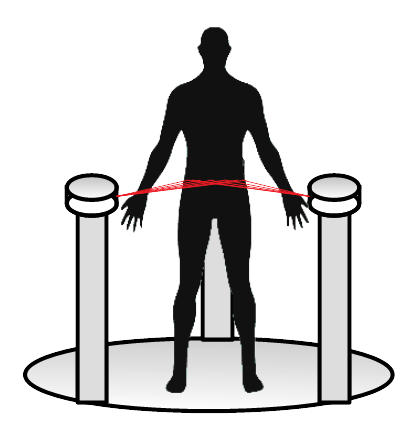
\includegraphics[height=6cm]{images/schematic_system.png}
    \caption[Simplified schematic of the system]{Simplified schematic of the system} {The user is surrounded by 3 poles and 3 LIDARs. Each LIDAR is mounted on a servomotor.}
    \label{fig:schematic_system}
\end{figure}

\begin{figure}[H]
    \centering
    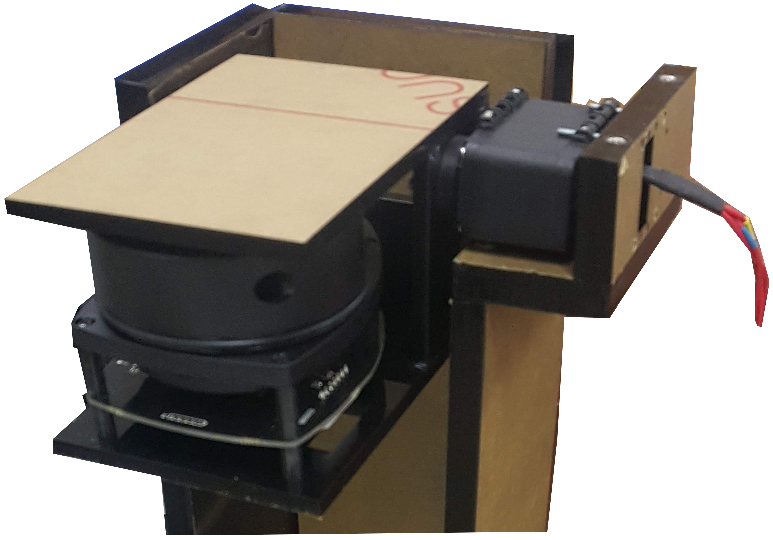
\includegraphics[height=6cm]{images/photo_pole_prototype.jpg} 
    \caption[Prototype of a pole]{Prototype of a pole}{We can see the servomotor which tilts the LIDAR.}
    \label{fig:photo_pole_prototype}
\end{figure}

To be able to aim at the user's navel (the level at which the measurement should be made), the LIDARs are mounted on a servomotor each which are on the top of a pole.   

\vsp

Then, a micro-controller control the actuators and sensors, compute the circumference and send the result to an interface. 

\subsection{Specifications}

The system must be:
\begin{itemize}
    \item Automatic: no need any user operation to perform the measurement
    \item Low cost: not much more hardware than described in the section \ref{sec:general_design}
    \item Fast: a maximum of a few seconds of measurement and computation
\end{itemize}

\vsp

Considering the mechanic part built-up and functional, the list above explains the tasks that should be done to make the system able to work properly: 
\begin{itemize}
    \item Controlling 3 servomotors and 3 LIDARs with a raspberry Pi, making them working together
    \item Study how to find the user's belly level
    \item Implementing the algorithm for user's circumference measurement from a point cloud
    \item Integrating the work in a program to control the machine and send the result to a computer via a serial com.
\end{itemize}

\section{Hardware implementation}

This project uses a Raspberry Pi v3, 3 RpLidar AX1, 3 and AX12 servomotors as described on the figure \ref{fig:basic_architecture}.

\begin{figure}[H]
    \centering
    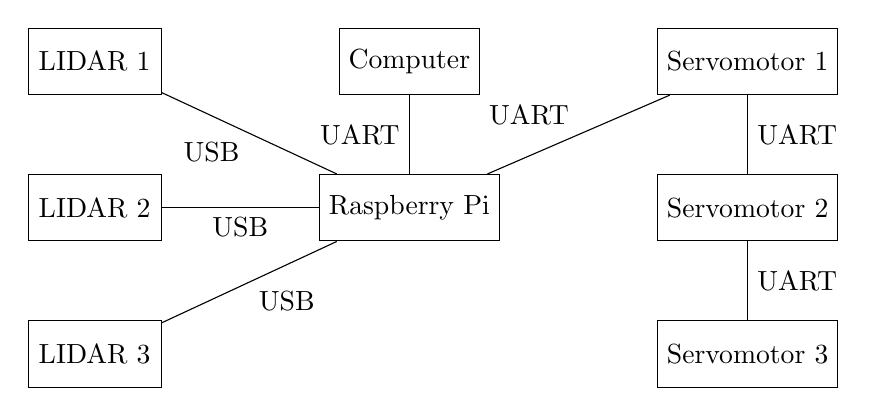
\begin{tikzpicture}[auto]
        \node[entity] (ras) {Raspberry Pi};
        \node[entity] (lid1) [above left = 1cm and 2cm of ras] {LIDAR 1};
        \node[entity] (lid2) [below = 1cm of lid1] {LIDAR 2};
        \node[entity] (lid3) [below = 1cm of lid2] {LIDAR 3};
        \node[entity] (ser1) [above right = 1cm and 2cm of ras] {Servomotor 1};
        \node[entity] (ser2) [below = 1cm of ser1] {Servomotor 2};
        \node[entity] (ser3) [below = 1cm of ser2] {Servomotor 3};
        \node[entity] (pc) [above = 1cm of ras] {Computer};
        \path (ras) edge node {USB} (lid1);
        \path (ras) edge node {USB} (lid2);
        \path (ras) edge node {USB} (lid3);
        \path (ras) edge node {UART} (ser1);
        \path (ser1) edge node {UART} (ser2);
        \path (ser2) edge node {UART} (ser3);
        \path (ras) edge node {UART} (pc);
    \end{tikzpicture}
    \caption{Basic architecture of the developed system}
    \label{fig:basic_architecture}
\end{figure}

\subsection{Raspberry Pi}

The Raspi's GUI is reached through a VNC server, connected to Eduroam. To find its IP address, use \textit{IP Finder}. A monitor can also be plugged to the HDMI port. 

\vsp

The program is integrally written in Python 3.6.

\subsection{LIDARs}

The open source library: \url{https://github.com/Roboticia/RPLidar} is used to control the LIDARs. While scanning, the 3 LIDARs gather the data alternately. They just need to be plugged to the raspberry pi in via USB.

\subsection{Servomotors}

The project uses the following open source library to control the servomotors:\url{https://pypi.org/project/pyax12/}. 

\vsp

The AX12 servomotors can be used in a daisy chain configuration. They have only 3 pins (2 for POWER and 1 for UART), which means that the RX/TX signals have to be multiplexed/demultiplexed in order to establish the communication. Thus, a simple circuit was designed as shown on the figure \ref{fig:elec_sch_servos}. 

\begin{figure}[H]
    \centering
    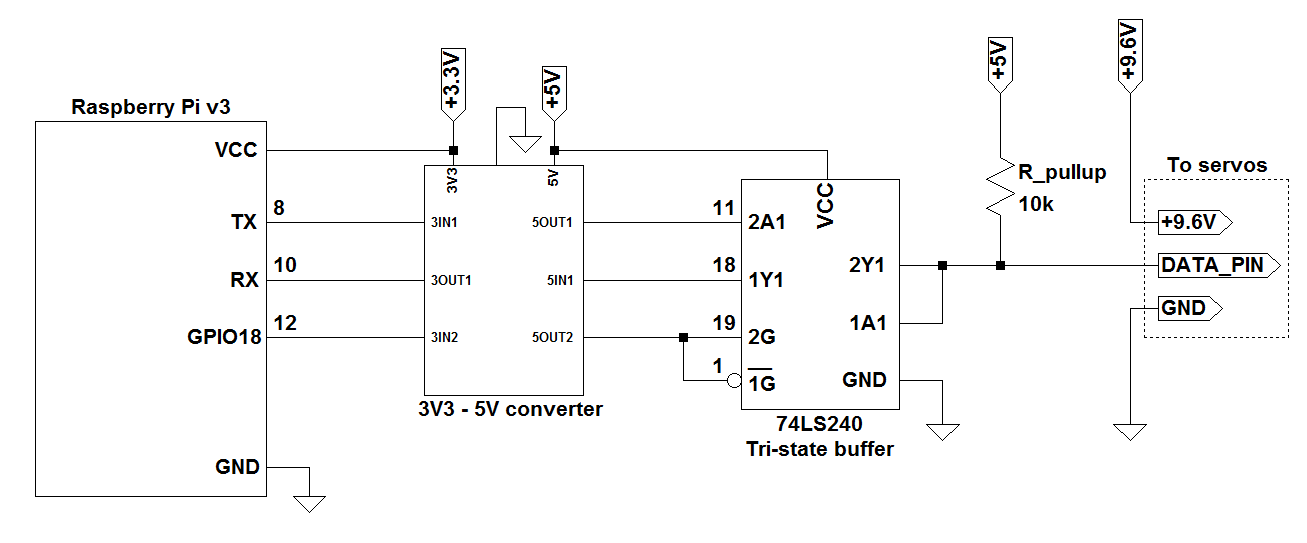
\includegraphics[width = \textwidth]{images/elec_sch_servo.png}
    \caption{Electronic circuit diagram for the servomotors' control}
    \label{fig:elec_sch_servos}
\end{figure}


Here, a 74LS240 tri-state buffer is used. It allows to control the direction of the communication with a single GPIO from the Raspi. When it is high, the Raspi can send data, when it is low, it receives the data. 

\vsp

To control the servomotors, few details need to be known:
\begin{itemize}
    \item The ideal baudrate is 57600
    \item Each servo as an ID and they must all be different
    \item When they all run at the same time, an high current drain can occur. Thus, without a powerful generator and high value capacitance, the speed should be set slow.
\end{itemize}

To configure the servomotors, a script is available in the source. It allows to test a servomotor by changing its position, to display all the servos' information, to set the max angles values, to change the rotation speed, to set the IDs and to configure the baudrate to 57600 with a brute-force algorithm. The servomotors should be configured with this program before using it in the project.


\section{Body scan}

The following section describes the procedure to scan a level of the body. For now we don't need to detect the navel, we just need to know where to scan at.

\subsection{Notations and physical quantities} \label{sec:notations}

Since now and until the end of this section, the norm an names described below will be used. 

\vsp

First, the units used are \textit{millimeters} and \textit{degrees}.

\vsp

The figure \ref{fig:top_view_system} is a top view of the system. The origin of the system frame in \textcolor{blue}{blue} is the middle of the base, represented by the circle. Since the lidar lie in a circle with $D$ as radius, the angle $\{ \beta_1,\ \beta_2,\ \beta_3 \}$ are the angles of the LIDARs from the origin vector $X$. In our case:
$$
\begin{bmatrix}
    \beta_1 &
    \beta_2 & 
    \beta_3 
\end{bmatrix}
=
\begin{bmatrix}
    \cfrac{ \pi}{6} &
    \cfrac{5\pi}{6} & 
    \cfrac{9\pi}{6} 
\end{bmatrix}
$$

\vsp

Each lidar has its own local frame represented in \textcolor{yellow}{gold}, and $\alpha$ is the angle between the $Y$ vector of the local frame (oriented to the middle of the circle) and the measured laser beam. $m$ is the distance of the between the laser beam source and the impact.

\vsp

The red zone inside the circle is a non-measurable area. Indeed, the lidars need a minimum distance to be able to perform a measurement. Moreover, the more this red zone is large, the wider the range of reachable scan heights. $d$ is the radius of the dead zone.

\vsp

Note that in this case, $\alpha < 0$ and $\beta < 0$.


\begin{figure}[H]
    \centering
    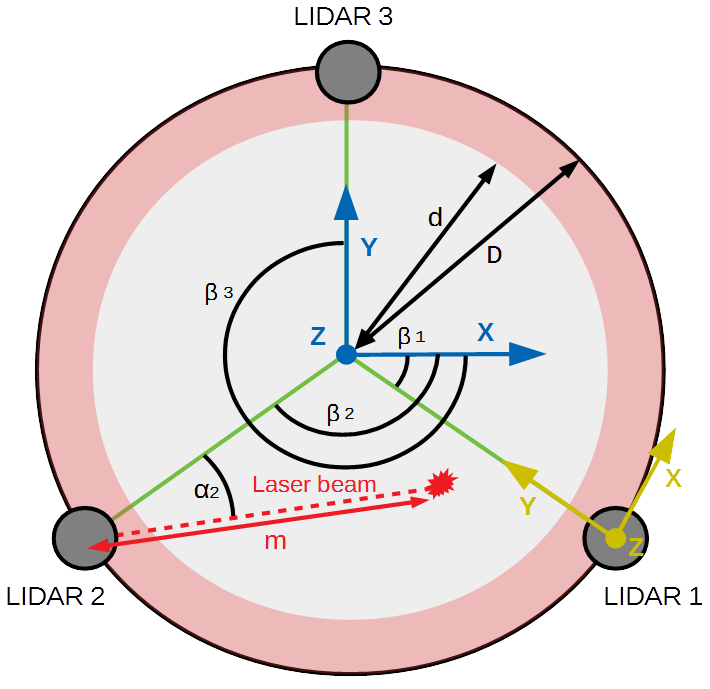
\includegraphics[width=10cm]{images/top_view_system.png}
    \caption{Top view of the system}
    \label{fig:top_view_system}
\end{figure}

The figure \ref{fig:side_view_system} shows a side view of the system. We can see that a servomotor is tilting the lidar and the angle between the zeroing (LIDAR in flat position) and the tilting is called $\theta$. Note that again in this case, $\theta < 0$.

\begin{figure}[H]
    \centering
    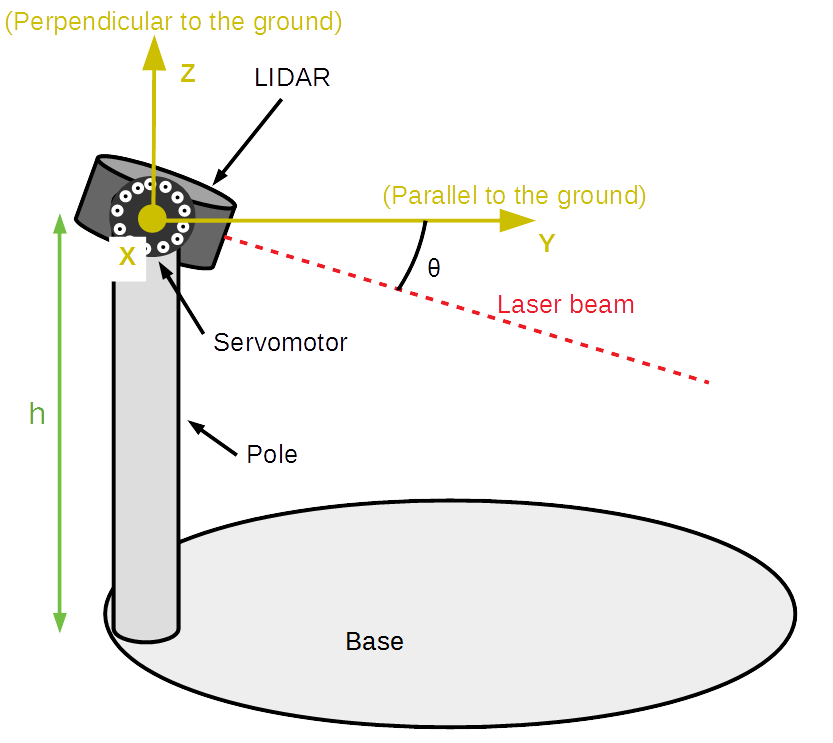
\includegraphics[width=10cm]{images/side_view_system.png}
    \caption{Side view of the system}
    \label{fig:side_view_system}
\end{figure}

\vsp

Finally, $h$ is the height of the lidar relative to the base. It is important because the origin of the altitude is at the base level.

\subsection{Scanning procedure}

Let's assume in this section that we want to perform a scan at an height $\Tilde{h}$. 

\vsp

The figure \ref{fig:cut_cylinder} intuitively shows the main problem that occurs when the lidar is higher or lower than the desired part of the body to scan. If we assume the human body as a cylinder, we can see that the lidar will measure the body at different height instead of the one desired.  

\begin{figure}[H]
    \centering
    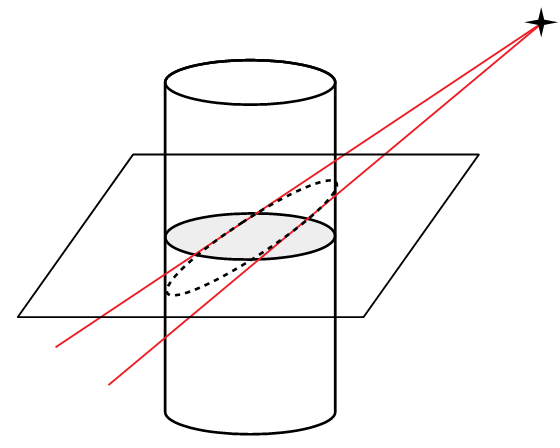
\includegraphics[height=6cm]{images/cut_cylinder.png}
    \caption{Cylinder cut from an higher source}
    \label{fig:cut_cylinder}
\end{figure}

To overpass this issue, a protocol has been implemented. It consists basically into tilting the lidar at many different angles, and to flatten the data measured close to the height $\Tilde{h}$.   

\vsp

The figure \ref{fig:sch_scanning_procedure} is a side view of the system, showing the lidar mounted on the pole on the left and the base at the bottom. The algorithm \ref{alg:scan_algo} describes the different steps of the scanning process.

\begin{figure}[H]
    \centering
    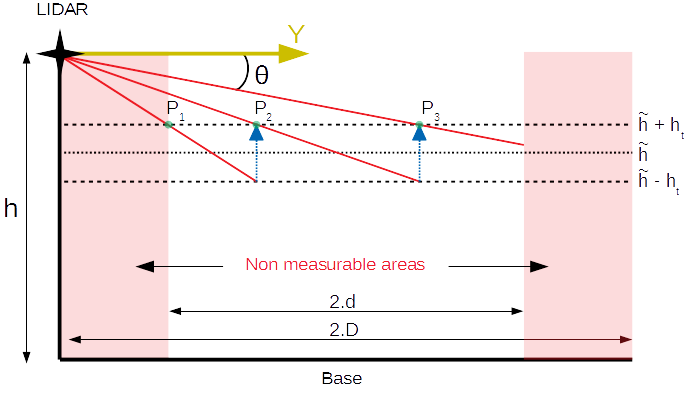
\includegraphics[width=\textwidth]{images/schematic_scan_procedure.png}
    \caption{Side view of the system with scanning procedure explanation}
    \label{fig:sch_scanning_procedure}
\end{figure}

The figure \ref{fig:sch_scanning_procedure} shows a tolerance zone around the desired height measurement $\Tilde{h}$ at levels $\Tilde{h}+h_t$ and $\Tilde{h}-h_t$. All this tolerance zone should be covered horizontally by the set of scans. By reading the figure \ref{fig:sch_scanning_procedure}, the process is as follows:

\begin{enumerate}
    \item Compute $P_1$, the intersect of the tolerance surface $\Tilde{h}+h_t$ vertically and the beginning of the measurable area horizontally.
    \item \label{alg:loop_step} Compute the intersection of a laser beam passing through $P_1$ which would intersect the inferior tolerance surface at level $\Tilde{h}-h_t$.
    \item Vertically project the point crossing the laser beam and the inferior tolerance surface on the superior tolerance surface to get $P_2$.
    \item Repeat the process from point $P_2$ since the step \ref{alg:loop_step} while $P_n < 2.D - (D-d) = D+d$.
    \item Scan the body with the angle corresponding to make the laser beam passing through the points $P_i$ found.
\end{enumerate}

\begin{algorithm}[H]
    \caption{Pseudo code of the scanning procedure}
    \label{alg:scan_algo}
    
    \hspace*{\algorithmicindent} \textbf{Input:} $h,\ \Tilde{h},\ h_t \in \mathbb{R}^+ $ \\
    \hspace*{\algorithmicindent} \textbf{Output:} $\theta_{arr}$ \ // \textit{Array that represents the pattern of angles to follow sequentially}
    \begin{algorithmic}[1]
        \STATE $\theta_{arr} \leftarrow [\ ]$
        \IF {$h \leq \Tilde{h}+h_t \ and \ h \geq \Tilde{h}-h_t $}
            \RETURN  $[0]$
        \ENDIF 
        \IF {$ h \geq \Tilde{h}+h_t $}
            \STATE $h_1 \leftarrow \Tilde{h}+h_t-h$, $h_2 \leftarrow  \Tilde{h}-h_t-h$
        \ELSE
            \STATE $h_1 \leftarrow \Tilde{h}-h_t-h$, $h_2 \leftarrow  \Tilde{h}+h_t-h$
        \ENDIF
        \STATE $d_1,\ d_2 \leftarrow D-d$
        \WHILE {$d_2 < d+D$}
            \STATE $new\_theta \leftarrow Atan2(h_1,d_1)$
            \STATE $\theta_{arr}.append(new\_theta)$
            \STATE $d_2 \leftarrow \cfrac{h_2}{Tan(new\_theta)}$
        \ENDWHILE
        \RETURN $\theta_{arr}$
    \end{algorithmic}
\end{algorithm}


\subsection{Finding the user navel's height}

Two different approach could be used to find the height of the user's navel: scanning the whole or a part of his body and detecting it, or estimating it through a statistical analysis.

\subsubsection{Detecting the navel's height}

Before implementing the detection, we need to know whether the degree of accuracy of our sensors and actuators. First, the datasheets of the LIDARs and servomotors give:

\begin{itemize}
    \item Servomotors' resolution: $\frac{330}{1024}^\circ = 0.322^\circ$
    \item LIDARs' distance resolution: $<0.5\ mm$ 
    \item LIDARs' angular resolution: $\leq 1^\circ$ 
\end{itemize}

We will consider the uncertainty of measurement of the Servomotors' position and the LIDARs' distance as negligible. However, let's compute the uncertainty $u$ of the LIDARs' angle measurement:

\begin{equation}
    u = \cfrac{angular\_resolution/2}{\sqrt{3}}\ deg = \cfrac{0.5}{\sqrt{3}}\ deg
\end{equation}

We choose to divide the half of the angular resolution by $\sqrt{3}$ as the measurement is likely made by a rotary encoder, giving measurements following an uniform probability distribution.

\vsp

Let $v=[d,0]$ be the measured vector in 2D space with $d$ the measured distance by the LIDAR, the uncertainty of position $u_p$ is given by:

\begin{equation}
        u_p = \sqrt{\big[ d - d.cos(u) \big] ^2 + \big[ -d.sin(u) \big] ^2}
\end{equation}

Then, the expanded uncertainty $U_p = k.u_p$ with $k$ the coverage factor. $k=1.96$ for a level of confidence of 95\%. Assuming for example, that the user is 500mm away from the LIDAR ($d=500$), then $U_p=5.0mm$. Simulation have been made and are shown on the figure \ref{fig:sim_navel_detection}. 

\begin{figure}[H]
    \centering
    \subfloat[Favourable conditions (width=10mm, depth=10mm, 150 data points)] {
        \label{fig:sim_navel_detection_favourable_case}
        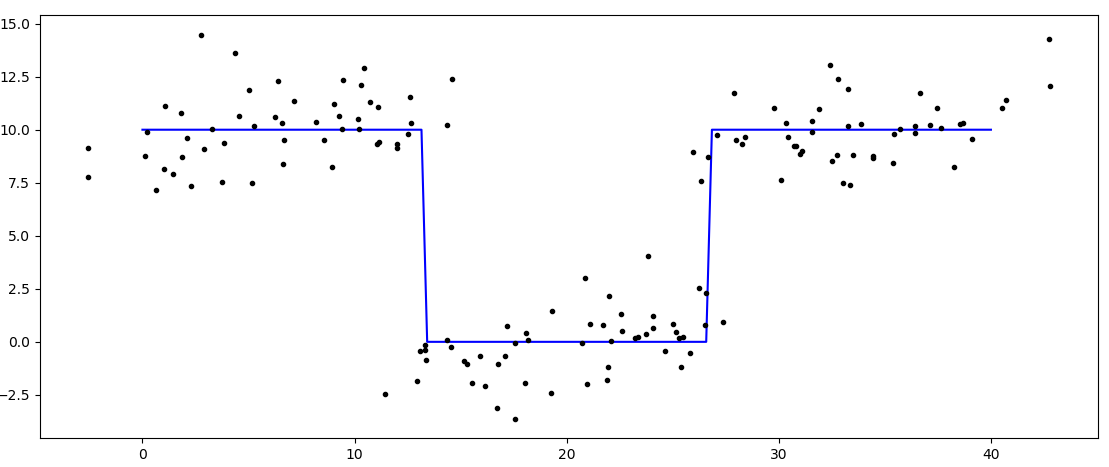
\includegraphics[width=8cm]{images/navel/detection/favourable_case.png}
        }
        \\
    \subfloat[Bad conditions (width=5mm, depth=5mm, 30 data points)] {
        \label{fig:sim_navel_detection_worse_case}
        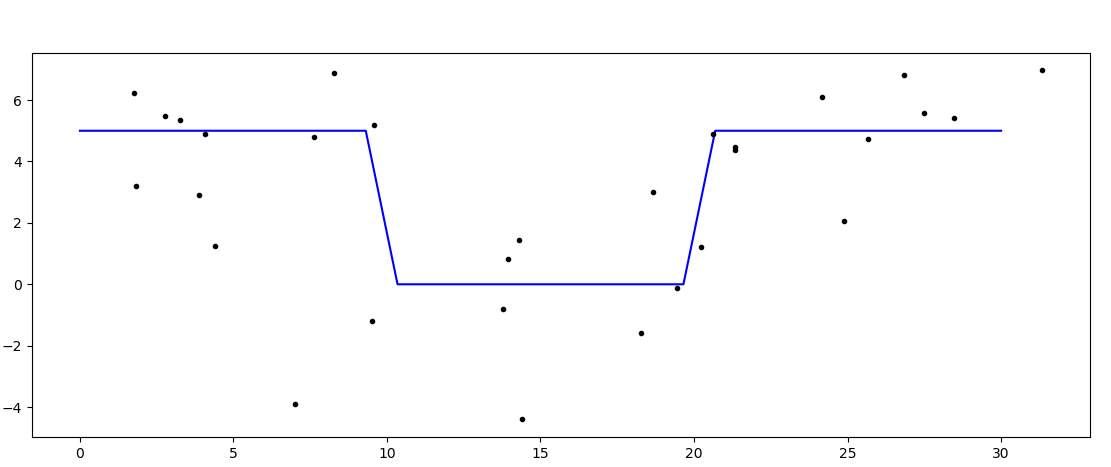
\includegraphics[width=8cm]{images/navel/detection/worse_case.png}
        } 
    \caption{Simulations of the user's navel detection}
    \label{fig:sim_navel_detection}
\end{figure}

The main problems with detecting the users' navel are cited below:

\begin{itemize}
    \item The characteristics of each nave are highly different for each person
    \item If the navel is too small or not depth enough, the data become too noisy
    \item It required a lot of time to scan a part of the body with LIDAR
    \item If the patient is short or tall compare to the pole, then the navel is not aligned with horizontally with the LIDAR
    \item It can cause some user inconvenience because he must not move at all and must not inflate his waist while breathing during the detection
\end{itemize}

For these reasons, the detection algorithm has not been implemented

\subsubsection{Estimating the navel's height}

A estimation of the navel's height was tried, based on other anthropomorphic parameters such as stature, weight and age. Two open databases have been used: one for children from the \textit{United States Consumer Product Safety Commission} \cite{database_cpsc_children} and another from the \textit{United States Army} for adults \cite{database_ansur2}. They both gathered data from both genders. 

\vsp

The figure \ref{fig:estimation_navel_various_parameters} shows the thousands of measurement and the height of the navel depending of the patients' stature (height), their weight and age. 

\begin{figure}[H]
    \centering
    \subfloat[Navel's height depending on patient's stature] {
        \label{fig:estimation_navel_depending_stature}
        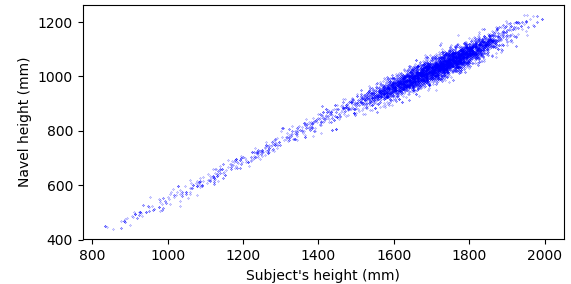
\includegraphics[width=8cm]{images/navel/estimation/navel_stature.png}
        }
    \subfloat[Navel's height depending on patient's weight] {
        \label{fig:estimation_navel_depending_weight}
        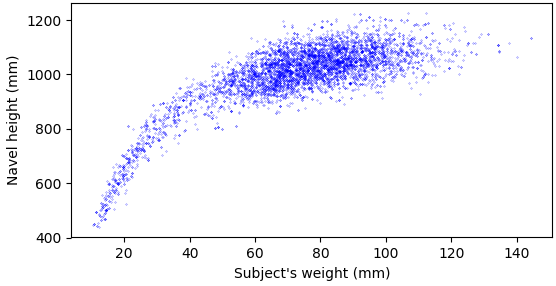
\includegraphics[width=8cm]{images/navel/estimation/navel_weight.png}
        } \\
    \subfloat[Navel's height depending on patient's age] {
        \label{fig:estimation_navel_depending_age}
        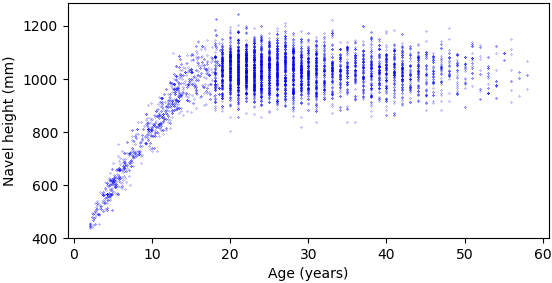
\includegraphics[width=8cm]{images/navel/estimation/navel_age.png}
        } 
    \caption{Patient's navel height depending on their stature, weight and age.}
    \label{fig:estimation_navel_various_parameters}
\end{figure}

Intuitively, we can notice a correlation between the navel's height and each of the parameters. If we compute the correlation coefficient $r$ described in the equation \ref{eq:correlation_coef}, we get the table \ref{tab:correlation_various_variables}.

\begin{equation}
\label{eq:correlation_coef}
    r = \cfrac{Cov(X,Y)}{\sigma_X \sigma_Y}
\end{equation}

$X$ and $Y$ are the variables and $\sigma_X$ and $\sigma_Y$ their standard deviation. Moreover $r \in [-1,1]$.

\begin{table}[H]
    \centering
    \begin{tabular}{|l|c|c|c|c|}
        \hline 
        Correlation (\%) & Stature & Weight & Age 
        \\ \hline
        Navel's height & $98\%$ & $79\%$ & $50\%$
        \\ \hline
        Stature & $/$ & $84\%$ & $54\%$
        \\ \hline
        Weight & $/$ & $/$ & $61\%$
        \\ \hline 
    \end{tabular}
    \caption{Correlation of various anthropomorphic data among each others}
    \label{tab:correlation_various_variables}
\end{table}

As the 4 variables are all pretty well dependant to each other, a multi-layered perceptron has been tested (provided by the \textit{sickit-learn} library) to estimate the navel's height. Moreover, as the correlation coefficients of the navel's height with the weight and stature is higher, a 2D linear regression has been implemented. Finally, a simple linear regression between the navel's height and stature has been tried. 

\vsp

By splitting the set of data into two groups, we can use a first part to train the regression while the other part is used to test the regression. 
\vsp

The error in $\epsilon_\%$ of the estimated navel's height for each test data is computed as follow:

\begin{equation}
    \epsilon_\% = \cfrac{\abs{\text{estimated - true}}}{\text{stature}}.100
\end{equation}

The error is thus given as a portion of the patient's stature. The errors found for each 3 methods are given below:

\begin{itemize}
    \item Multi-layer perceptron: 1.21\% 
    \item 2D linear regression stature/weight: 1.04\% 
    \item Linear regression on the stature: 0.94\%
\end{itemize}

As the simple linear regression shows the best results, we use this method and the error terms of a set of test are shown in figure \ref{fig:distrib_estimated_navel} in a distribution graph.

\begin{figure}[H]
    \centering
    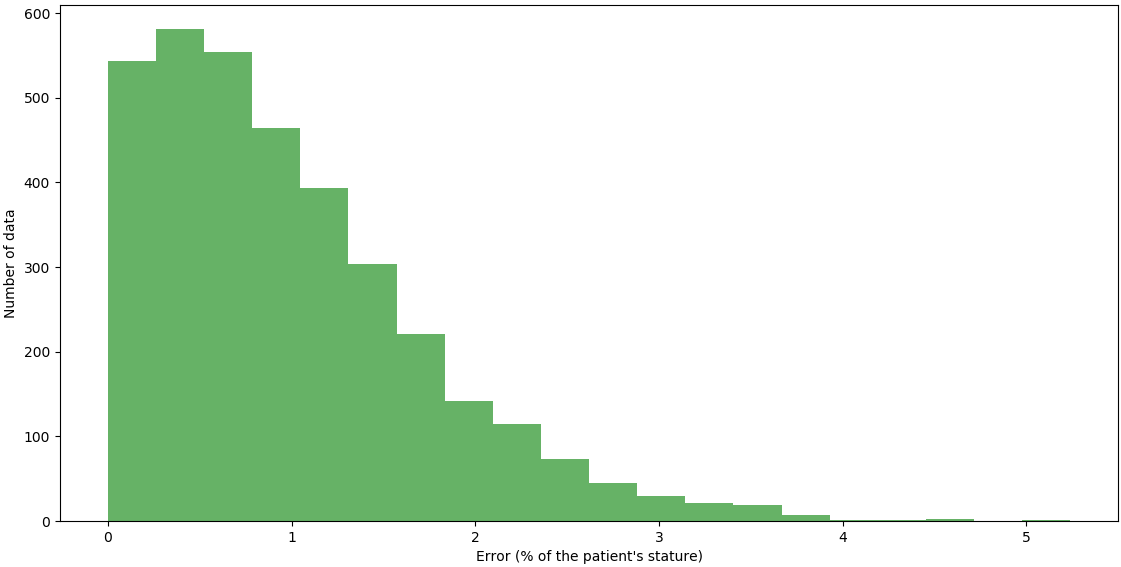
\includegraphics[width=12cm]{images/navel/estimation/distrib_estimated_navel.png}
    \caption{Distribution of the estimated navel height's error}
    \label{fig:distrib_estimated_navel}
\end{figure}

All the results are presented in the table \ref{tab:results_error_estimated_navel} and are interpolated for people 140cm, 160cm and 180cm tall:

\begin{table}[H]
    \centering
    \begin{tabular}{|l|c|c|c|c|}
        \hline 
        Error: & Fraction of the stature & 140cm tall patients & 160cm tall patients & 180cm tall patients 
        \\ \hline
        Mean & $0.94\%$ & $13.16$mm & $15.04$mm & $16.92$mm 
        \\ \hline
        Median & $0.83\%$ & $11.62$mm & $13.28$mm & $14.94$mm 
        \\ \hline
        75-percentile & $1.39\%$ & $19.46$mm & $22.24$mm & $25.02$mm 
        \\ \hline
        95-percentile & $2.40\%$ & $38.40$mm & $38.40$mm & $43.20$mm 
        \\ \hline
        Max error & $5.24\%$ & $73.36$mm & $83.84$mm & $94.32$mm 
        \\ \hline 
    \end{tabular}
    \caption{Error of the estimated navel's height}
    \label{tab:results_error_estimated_navel}
\end{table}

Note that the database used are not sampling a good representation of the population (soldiers and American children). Some other set of data more adapted to global population may be found. 

\subsection{Running a scan}

The 3 LIDARs have to scan in parallel. However, only one thread is running at the same time. It means that the program gathers the measurements one by one on each LIDAR. Moreover, the servomotors are all moving at the same time to avoid too much distortions if the users moves during the scan. Once the Raspi has yielded the measurements, it saves them into text files containing the angle of rotation of the lidar $\alpha$, the angle of tilting of the servomotors $\theta$ and the distance from the measured object $m$, giving a file containing: 
$$ 
\begin{bmatrix}
    \alpha_{j} & \theta_{j} & m_{j} 
\end{bmatrix}_i
$$
with $i$ number of LIDARs and $j$ number of measurements. Another file contains the scan's information (for now, only the height $\Tilde{h}$) 


\subsection{Raw data to point cloud}

Once the scan is over, 3 text files and 1 info file have been generated. The goal now is to locate every measurement in the 3D space.

\vsp

Each measurement is a 3D vector, having the LIDAR as origin. Let's find the orientation of the vector for each measurement of the LIDAR $i$. $m$ is the norm of the vector, and is the distance measured by the LIDAR. In the LIDAR's frame as shown in the figure \ref{fig:top_view_system} and figure \ref{fig:side_view_system}, let's assume the vector $v_{0,j} = 
\begin{bmatrix}
0 & m_j & 0 
\end{bmatrix}$, which mean a vector having the LIDAR as origin and pointing forward.

\vsp

Now we want to rotate it with the rotation matrix given in \cite{rot_mat_euler}. The elemental rotation matrices around the axis X and Z can be expressed as follow:

\begin{equation}
\label{eq:rot_mat_x}
    R_X(\theta_j) = 
    \begin{bmatrix}
        1 & 0 & 0 \\
        0 & cos(\theta_j) & -sin(\theta_j) \\
        0 & sin(\theta_j) & cos(\theta_j)
    \end{bmatrix}
\end{equation}

\begin{equation}
\label{eq:rot_mat_y}
    R_Z(\alpha_j) = 
    \begin{bmatrix}
        cos(\alpha_j) & -sin(\alpha_j) & 0 \\
        sin(\alpha_j) & cos(\alpha_j) & 0 \\
        0 & 0 & 1
    \end{bmatrix}
\end{equation}

Moreover, we need to get the final vector in the system's frame. To transform the LIDAR's frame into the system's frame, we will rotate the around Z-axis by $+90^\circ$ (to match the X and Y axis) and then rotate it again around the Z-axis by the value of its position angle $\beta_i$. 

\vsp

Thus, the final rotation matrix can be written by combining \ref{eq:rot_mat_x} and \ref{eq:rot_mat_y}:

\begin{equation}
    R_{final}(\beta_i,\theta_j,\alpha_j) = 
    R_Z(\beta_i+90^\circ).R_X(\theta_j).R_Z(\alpha_j) =
    \begin{bmatrix}
        c_1c_3 - c_2s_1s_3 & -c_1s_3-c_2c_3s_1 & s_1s_2 \\
        c_3s_1 + c_1c_2s_3 & c_1c_2c_3-s_1s_3 & -c_1s_2 \\
        s_2s_3 & c_3s_2 & c_2
    \end{bmatrix}
\end{equation}

For readability purpose, $c$ means $cos$ and $s$ means $sin$, while $1$ correspond to $\beta_i+90^\circ$, $2$ to $\theta_j$ and $3$ to $\alpha_j$. For instance, $c2$ means $cos(\theta_j)$.

\vsp

We obtain:
\begin{equation}
    v_j^T = R_{final}(\beta_i,\theta_j,\alpha_j).v_{0,j}^T = m_j.
     \begin{bmatrix}
        -c_1s_3-c_2c_3s_1\\
        c_1c_2c_3-s_1s_3 \\
        c_3s_2
    \end{bmatrix}
\end{equation}

So, $v_j$ is the vector in the system frame having the system origin as starting point. A simple shift can be apply to it depending on the position of the LIDAR. The point $P_j$ is the 3D measurement $j$ made by the LIDAR $i$:

\begin{equation}
\label{eq:point_computation}
    P_j = v_{0,j}^T + 
    \begin{bmatrix}
        D.cos(\beta_i) \\
        D.sin(\beta_i) \\
        h
    \end{bmatrix}
\end{equation}

It could be enough in theory but practically, the system looks more like presented on figure \ref{fig:prototype_tilting}. When the LIDAR is tilted, its position changes.

\begin{figure}[H]
    \centering
    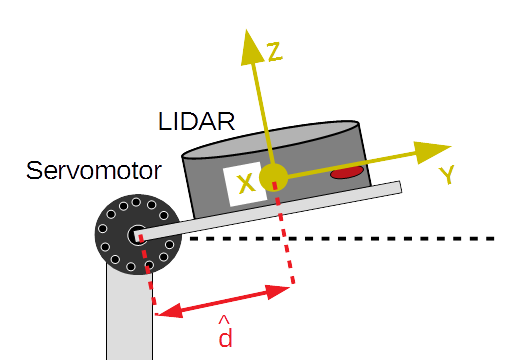
\includegraphics[height = 6cm]{images/bias_real_system.png}
    \caption{Mechanism of the LIDAR tilting of the prototype}
    \label{fig:prototype_tilting}
\end{figure}

Let's add to our equation \ref{eq:point_computation} a position correction with $\Hat{d}$ the distance between the center of rotation of the servomotor and the LIDAR. 

\begin{equation}
    P_j = v_{0,j}^T + 
    \begin{bmatrix}
        D.cos(\beta_i) \\
        D.sin(\beta_i) \\
        h
    \end{bmatrix}
    +
    \begin{bmatrix}
    \Hat{d}.cos(\beta_i).(1-cos(\theta_j)) \\
    \Hat{d}.sin(\beta_i).(1-cos(\theta_j)) \\
    \Hat{d}.sin(\theta_j)
    \end{bmatrix}
\end{equation}

The figure \ref{fig:3D_cloud} shows an example of scanned 3D cloud.

\begin{figure}[H]
    \centering
    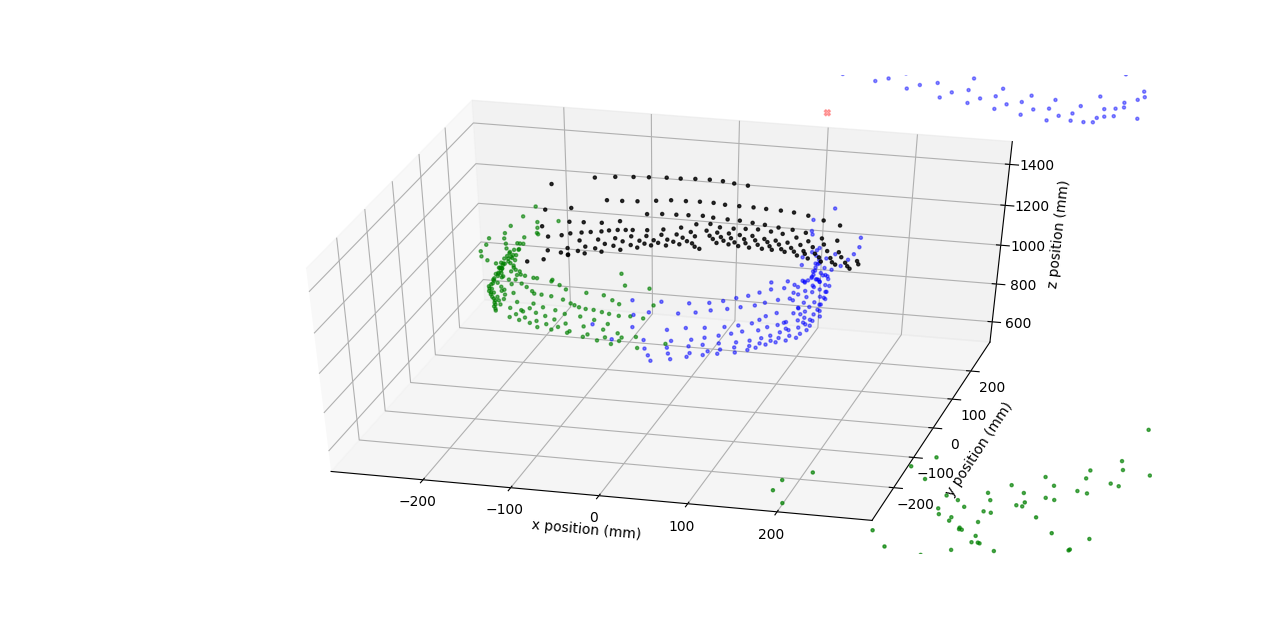
\includegraphics[height = 6cm]{images/3D_cloud.png}
    \caption[Example of 3D a point cloud]{Example of a 3D point cloud computed. Each color corresponds to a different LIDAR.}
    \label{fig:3D_cloud}
\end{figure}



\section{Contour reconstruction}

After flattening the points around $\Tilde{h}$, we get a 2D point cloud. The goal now is to compute a smooth curve that fits the data points.



\subsection{Presentation of the method}

The method chosen here is inspired by the Wang et al's paper \cite{SDM_bspline_fitting} which presents a method called \textit{Squared Distance Minimization} for computing a closed planar B-Spline curve that reconstructs the shape of a point cloud of non-ordered data. 

\vsp

A B-spline curve is a specific combination of splines which are themselves, functions defined piecewise by polynomials. The optimization process is a non linear least square problem and will be performed by minimizing an objective function. 

\vsp

Contrary to the LOESS based reconstruction that was first implemented in this project and presented in the Vincent MAIRE's report \cite{MAIRE_internship_report}, this method has been chosen mostly because it is well documented and many papers discuss about it. Thus, some improvements can be made more easily in the future.



\subsection{Sum up on B-spline}

A B-spline curve can be written: 
\begin{equation}
    \label{eq:bspline_definition}
    P(t)=\sum\limits_{i=1}^m B_{i,n}(t)P_i
\end{equation}

with $t$ the value of the knot, $m$ the number of control points, $B_{i,n}(t)$ the basis element of order $n$ at the knot $t$ and $P_i(t)$ the position of the control point $i$.

\vsp

A B-spline has an order, which defines how far a node will affect another from. In our case, we will use an order of 3 as it is the most common used and the author of the paper does not provide any further details about this.

\vsp

The B-spline is also set by a knot vector, which gives a value to each knot at each control point. A control point is the coefficient that, to sum up the equation \ref{eq:bspline_definition}, represents the position of the B-spline. If we consider a zero order B-spline, then the curve at the knot value $t_i$ will exactly pass through the value of $P_i$.

\vsp

A B-spline basis element is a recursive function defined by the equation:
\begin{equation}
    \begin{array}{c c}
        B_{i,0}(t) = 
        \left \{
        \begin{array}{l l}
            1 & if\ t_i \leq t < t_{i+1} \\
            0 & otherwise
        \end{array}
        \right .
        \\
        B_{i,n}(t) = \cfrac{t-t_i}{t_{i+n}-t_i}B_{i,n-1}(t) + 
                     \cfrac{t_{i+n+1}-t}{t_{i+n+1}-t_{i+1}}B_{i+1,n-1}(t)
    \end{array}
\end{equation}


\subsection{Method's steps} \label{sec:method_steps}

We assume that the number of control points and the order of the spline will stay the same. This method consists in translating the control points at every step.

\vsp

The first step is to find a good initial B-spline curve which fits with the data, since this method is highly dependent to the initial conditions.

\vsp

The fitting B-spline can be written from the equation \ref{eq:bspline_definition}: $P_c(t)=\sum\limits_{i=1}^m B_i(t)P_{c,i}$. Let $P_+$ be the updated B-spline after moving the control points as $P_+=P_c+D$. Then, we will define as a \textit{footpoint} the closest point $P_c(t_k)$ of the curve to the data point $X_k$. $T_k$, $N_k$ and $\rho$ are respectively the tangent unit vector, the normal unit vector and the curvature radius of the curve $P_c(t)$ at the point $P_c(t_k)$. $d$ is the signed distance as $\abs{d} = \left\lVert P_c(t_k) - X_k \right\rVert$ and its sign is chosen following this rule: $d \geq 0$ if $X_k$ is on the same side of the curve curvature center at the point $P_c(t_k)$, $d < 0$ otherwise. 

\vsp

For each iteration of the algorithm, every of the described above characteristics must be computed. Now, let's define the error term named \textit{Squared Distance} as:
\begin{equation}
    \label{eq:error_term}
    e_{SD,k}(D) = 
    \left \{
    \begin{array}{l l}
        \cfrac{d}{d-\rho}[(P_+(t_k)-X_k)^T T_k]^2 + [(P_+(t_k)-X_k)^T N_k]^2 & if\ d < 0 \\
        \big[(P_+(t_k)-X_k)^T N_k\big]^2 & if\ 0 \leq d < \rho 
    \end{array}
    \right .
\end{equation}

By computing at each iteration the Squared Distance error term for every data point, we obtain the $f_{SD}$ term that we will minimize as:
\begin{equation}
    \label{eq:fsd}
    f_{SD} = \cfrac{1}{2} \sum_{k} e_{SD,k} + \lambda f_s
\end{equation}

Here, $f_s$ is a regularization term to improve the stability and $\lambda$ is a pondering coefficient. The $f_{SD}$ is quadratic and thus, can be minimized by solving a linear system of equations. Then an incremental change of $D$ to the initial control points is applied.

\vsp

The process can be iterated until a user custom error term is below a threshold or if the incremental change $D$ becomes small enough.


\subsection{Implementation}

This section describes how this method has been implemented for our system, what could be improved.

\subsubsection{B-spline computing}

Actually, the program is written in Python, which provides libraries for B-spline computing (through \textit{Scipy}). Two are particularly interesting and their characteristics are presented in the table \ref{tab:bspline_lib}. In this project, these two functions have been used. 

\begin{table}[H]
    \centering
    \begin{tabular}{|l|p{10cm}|}
        \hline
        \textbf{scipy.interpolate.BSpline} &
        \textbullet ~ Create a 1D open B-spline function object from the knots, control points and order \newline
        \textbullet ~ Evaluate the value, the derivative and integral of the B-spline at $t$ \newline
        \textbullet ~ Return the basis element of the B-spline at $t$
        \\
        \hline
        \textbf{scipy.interpolate.splprep} & 
        \textbullet ~ Create a 2D open or closed interpolation B-spline object from an ordered list of points
        \\
        \hline 
    \end{tabular}
    \caption{Two interesting B-spline computing libraries provided by Scipy}
    \label{tab:bspline_lib}
\end{table}

To compute a B-spline, \textbf{scipy.interpolate.BSpline} is called twice, in order to generate a B-spline on both $x$ and $y$ axis. Then the values on both axis are evaluated independently. 

\vsp

Then, to be make the B-spline periodic as we want to reconstruct a closed shape, it is necessary to append the $n$ first knot values and coefficients to the B-spline knot values and coefficient. That way, the B-spline will repeat its last values as if it was closed.

\subsubsection{Finding the initial spline}

As said in the section \ref{sec:method_steps}, an initial B-spline must be found before running the algorithm. The chosen implementation here is a circle fitting, since the human shape is quite circular and symmetric about the two axis.

\vsp

The least square fitting method as described in the Dumbach et al 's paper \cite{circle_fitting} is used, computing the radius and position with the equations \ref{eq:circle_fitting}.

\begin{equation}
    \label{eq:circle_fitting}
    \begin{aligned}
        A &= n \sum \limits_{j=1}^{n}x_j^2 - 
        \bigg( \sum \limits_{j=1}^{n} x_j \bigg) ^2
        \\[5pt]
        B &= n \sum \limits_{j=1}^{n}x_j y_j -
        \bigg( \sum \limits_{j=1}^{n} x_j \bigg)
        \bigg( \sum \limits_{j=1}^{n} y_j \bigg) 
        \\[5pt]
        C &= n \sum \limits_{j=1}^{n}y_j^2 - 
        \bigg( \sum \limits_{j=1}^{n} y_j \bigg) ^2
        \\[5pt]
        D &= 0.5 \bigg\{ 
        n \sum \limits_{j=1}^{n}x_j y_j^2 
        \bigg( \sum \limits_{j=1}^{n} x_j \bigg) \bigg( \sum \limits_{j=1}^{n} y_j^2 \bigg)
        + n \sum \limits_{j=1}^{n}x_j^3 - 
        \bigg( \sum \limits_{j=1}^{n} x_j \bigg)
        \bigg( \sum \limits_{j=1}^{n} x_j^2 \bigg)
        \bigg\} 
        \\[5pt]
        E &=  0.5 \bigg\{
        n \sum \limits_{j=1}^{n}y_j x_j^2 
        \bigg( \sum \limits_{j=1}^{n} y_j \bigg) \bigg( \sum \limits_{j=1}^{n} x_j^2 \bigg)
        + n \sum \limits_{j=1}^{n}y_j^3 - 
        \bigg( \sum \limits_{j=1}^{n} y_j \bigg)
        \bigg( \sum \limits_{j=1}^{n} y_j^2 \bigg)
        \bigg\}
        \\[10pt]
        a_M &= \cfrac{DC-BE}{AC-B^2}
        \\[5pt]
        b_M &= \cfrac{AE-BD}{AC-B^2}
        \\[5pt]
        r_M &= \frac{1}{n} 
        \sum \limits_{j=1}^{n}
        \sqrt{(x_j-a_M)^2+(y_j-b_M)^2}
        \\
    \end{aligned}
\end{equation}

With $x_j$ and $y_j$ the coordinates of the j-th point, $a_M$ and $b_M$ the position of the fitted circle's center and $r_M$ its radius. 

\vsp

Now that we have a circle that barely fits with the point cloud, we split it into $N_ctrl$, the number of control points of the B-spline, equal sections as shown in the figure \ref{fig:split_circle}. Let's assume moreover that it creates areas with infinite size as they grow even outside the circle.

\begin{figure}[H]
    \centering
    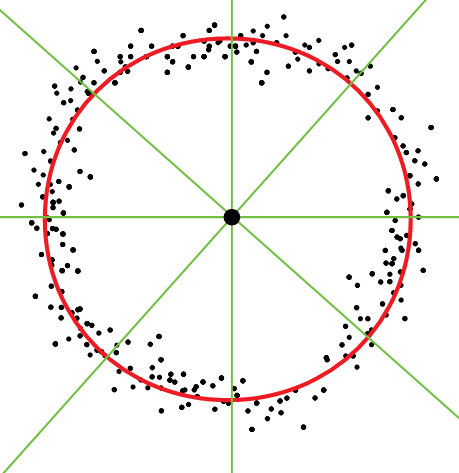
\includegraphics[height = 5cm]{images/circle_split.png}
    \caption[How to split the fitting circle]{How to split the fitting circle. Example with 8 control points.}
    \label{fig:split_circle}
\end{figure}

Then, the median of the distance of the points to the center is computed for each area, taking into account the points that lie in the concerned area. We use the median as it is more robust to outliers than averaging. Finally, since we need the value of the first control points, the function \textit{scipy.interpolate.splprep} is called to create an interpolation B-spline that fits the computed points. The control points of the initial B-spline are then extracted from this previous B-spline.

\vsp

In the case an area does not include any points, then we compute the average of the median of the two surrounding zones. If the surrounding zone do not include any points too, a linear interpolation is made between the two closest zone that contain points. 

\vsp

This method brought good results and becomes even more accurate when the number of control points increases. Some examples of the results for several number of control points $n$ are shown in figure \ref{fig:initial_fit_results}. 

\begin{figure}[H]
    \centering
    \subfloat[n=5] {
        \label{fig:bsp_res_init_n5}
        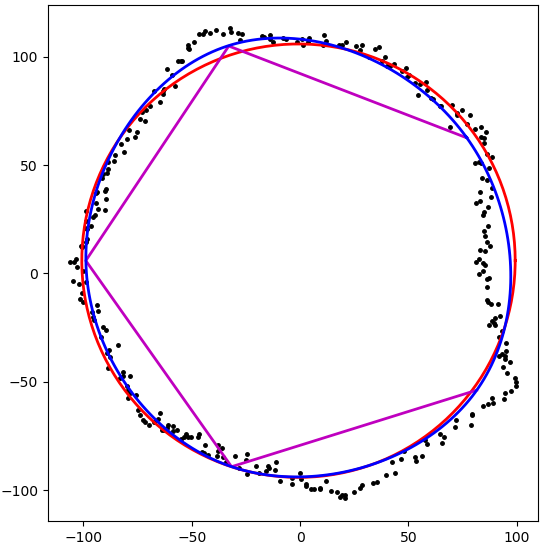
\includegraphics[width=5cm]{images/bsp_res/init/5n.png}
        }
    \subfloat[n=10] {
        \label{fig:bsp_res_init_n10}
        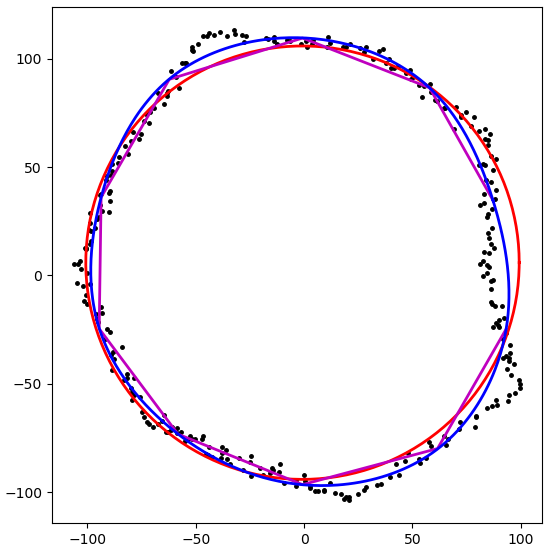
\includegraphics[width=5cm]{images/bsp_res/init/10n.png}
        } \\
    \subfloat[n=15] {
        \label{fig:bsp_res_init_n15}
        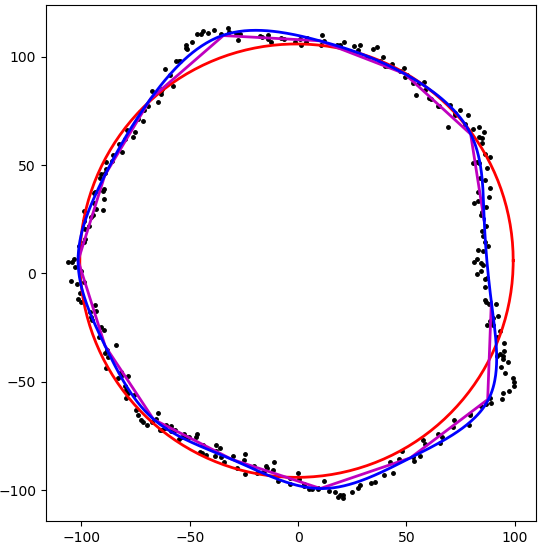
\includegraphics[width=5cm]{images/bsp_res/init/15n.png}
        } 
    \subfloat[n=20] {
        \label{fig:bsp_res_init_n20}
        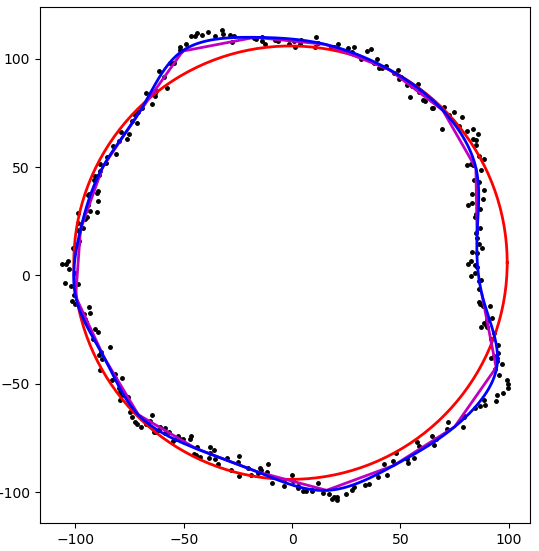
\includegraphics[width=5cm]{images/bsp_res/init/20n.png}
        } 
    \caption[Initial B-spline results]{Initial B-spline results. In \textcolor{red}{red}, the fitted circle, in \textcolor{magenta}{magenta} the distance median for each area and in \textcolor{blue}{blue} the initial B-spline found.}
    \label{fig:initial_fit_results}
\end{figure}


\subsubsection{Point's parameters computing}

Many different parameters should be computed for each point of each iteration as presented in the section \ref{sec:method_steps}.

\vsp

First, the footpoint which is the closest point $P_c(t_k)$ of the curve to the data point $X_k$ must be computed. Many different methods can be implemented. In our case, the following process is applied:

\begin{enumerate}
    \item Evaluating the B-spline with a large number of point (here 50 points per control node)
    \item Computing the distance of each point to each point of the evaluated curve 
    \item Finding the minimum distance and returning $t_k$ the knot value of the footpoint $P_c(t_k)$
\end{enumerate}

Then the tangent and normal vector can be recovered by derivating respectively once and twice the B-spline and dividing each $x$ and $y$ parameters by the vector's norm to make it unit.

\vsp

The radius $\rho$ of the curve at $t_k$ is the norm of the normal vector $N_k$. 

\vsp

To find the signed distance $d$, we compute $k=(X_k-P_c(t_k))^T N_k$. If the parameter of $k=[k_x,k_y]$ with the greatest value is negative, then $d < 0$, else $d \geq 0$. 


\subsubsection{Minimizing the objective function}

The function $f_{SD}$ described in the equation \ref{eq:fsd} must be minimized in order to find the optimal incremental update $D$. The implementation of the algorithm is inspired from the work of Pekelny \cite{pekelny_bsp} and Mhala \cite{mahla_bsp}.

\vsp

As shown in Wang et al 's paper \cite{SDM_bspline_fitting}, $f_{SD}$ is positive quadratic in $D_i$, which means that it can be minimized solving $\cfrac{\partial f_{SD}}{\partial D} = 0$. It can be written in the form $Ax=b$ as follow: 

\begin{equation}
\label{eq:axb}
    \begin{bmatrix}
    \Bigg( \cfrac{\partial f_{SD}}{\partial D_{1,x}} \Bigg) _{1,x} &
    \cdots &
    \Bigg( \cfrac{\partial f_{SD}}{\partial D_{1,x}} \Bigg) _{n,x} &
     &
    \Bigg( \cfrac{\partial f_{SD}}{\partial D_{1,x}} \Bigg) _{1,y} &
    \cdots &
    \Bigg( \cfrac{\partial f_{SD}}{\partial D_{1,x}} \Bigg) _{n,y} 
    \\
     & & & \vdots & & & 
    \\
    \Bigg( \cfrac{\partial f_{SD}}{\partial D_{n,x}} \Bigg) _{1,x} &
    \cdots &
    \Bigg( \cfrac{\partial f_{SD}}{\partial D_{n,x}} \Bigg) _{n,x} &
     &
    \Bigg( \cfrac{\partial f_{SD}}{\partial D_{n,x}} \Bigg) _{1,y} &
    \cdots &
    \Bigg( \cfrac{\partial f_{SD}}{\partial D_{n,x}} \Bigg) _{n,y} 
    \\
    \Bigg( \cfrac{\partial f_{SD}}{\partial D_{1,y}} \Bigg) _{1,x} &
    \cdots &
    \Bigg( \cfrac{\partial f_{SD}}{\partial D_{1,y}} \Bigg) _{n,x} &
     &
    \Bigg( \cfrac{\partial f_{SD}}{\partial D_{1,y}} \Bigg) _{1,y} &
    \cdots &
    \Bigg( \cfrac{\partial f_{SD}}{\partial D_{1,y}} \Bigg) _{n,y} 
    \\
     & & & \vdots & & & 
    \\
    \Bigg( \cfrac{\partial f_{SD}}{\partial D_{n,y}} \Bigg) _{1,x} &
    \cdots &
    \Bigg( \cfrac{\partial f_{SD}}{\partial D_{n,y}} \Bigg) _{n,x} &
     &
    \Bigg( \cfrac{\partial f_{SD}}{\partial D_{n,y}} \Bigg) _{1,y} &
    \cdots &
    \Bigg( \cfrac{\partial f_{SD}}{\partial D_{n,y}} \Bigg) _{n,y} 
    \end{bmatrix}_{2n,2n}
    \begin{bmatrix}
        D_{1,x} \\
        \vdots \\
        D_{n,x} \\
        D_{1,y} \\
        \vdots \\
        D_{n,y} 
    \end{bmatrix}_{1,2n}
    =
    \begin{bmatrix}
        b_{1,x} \\
        \vdots \\
        b_{n,x} \\
        b_{1,y} \\
        \vdots \\
        b_{n,y} 
    \end{bmatrix}_{1,2n}
\end{equation}

The left matrix is $A$, the middle is $x$ and the right is $b$, with $n$ the number of control points, $D$ the incremental update and $b$ the constant term of the derivative. Each term $\Bigg( \cfrac{\partial f_{SD}}{\partial D_{i,x/y}} \Bigg) _{j,x/y}$ must be computed, which is the coefficient of $D_{j,x/y}$ when $f_{SD}$ is derivated by $D_{i,x/y}$.

\vsp

With the equation \ref{eq:fsd}, we see that $f_{SD}$ is a combination of the error term $e_{SD}$ and the regularization term $f_s$. First, we do not consider the regularization term, thus:

\begin{equation}
    \cfrac{\partial f_{SD}}{\partial D_{i,x/y}} = 
    \frac{1}{2} \sum_{k} \cfrac{\partial e_{SD,k}}{\partial D_{i,x/y}}
\end{equation}

When $0 \leq d < \rho$, with the formula of $e_{SD}$ defined in the equation \ref{eq:error_term}:

\begin{equation}
\label{eq:derivative_esd_x_d_greater_0}
    \begin{aligned}
        e_{SD,k} & = [(P_+(t_k))-X_k)^T N_k]^2 
        \\[5pt]
        \cfrac{\partial e_{SD,k}}{\partial D_{i,x}} 
        & = \cfrac{\partial [(P_+(t_k))-X_k)^T N_k]^2}{\partial D_{i,x}} 
        \\
        & = 2\beta_i(t_k)N_{k,x}[(P_+(t_k)-X_k)^T N_k]
        \\
        & = 2\beta_i(t_k)N_{k,x}
        \Bigg[ \bigg( \sum \limits_{j=1}^{n} \beta_j(t_k)D_j \bigg) ^T N_k \bigg) \Bigg]
        + 2\beta_i(t_k)N_{k,x} [(P(t_k)-X_k)^T N_k]
        \\
        & = 2\beta_i(t_k)N_{k,x}^2 \sum \limits_{j=1}^{n} \beta_j(t_k)D_{j,x} 
        + 2\beta_i(t_k)N_{k,x}N_{k,y} \sum \limits_{j=1}^{n} \beta_j(t_k)D_{j,y} 
        + 2\beta_i(t_k)N_{k,x} [(P(t_k)-X_k)^T N_k]
    \end{aligned}
\end{equation}

In the same way as the equation \ref{eq:derivative_esd_x_d_greater_0}, we can find $\cfrac{\partial e_{SD,k}}{\partial D_{i,y}}$ when $0 \leq d < \rho$:

\begin{equation}
\label{eq:derivative_esd_y_d_greater_0}
    \cfrac{\partial e_{SD,k}}{\partial D_{i,y}} 
     = 2\beta_i(t_k)N_{k,y}^2 \sum \limits_{j=1}^{n} \beta_j(t_k)D_{j,y} 
    + 2\beta_i(t_k)N_{k,x}N_{k,y} \sum \limits_{j=1}^{n} \beta_j(t_k)D_{j,x} 
    + 2\beta_i(t_k)N_{k,y} [(P(t_k)-X_k)^T N_k]
\end{equation}

Now, when $d < 0$, the error term is very similar as it is the sum of the error term when $0 \leq d$ and itself when $N$ is replaced by $T$ times $\cfrac{d}{d-\rho}$. Thus, when $d < 0$, we have:

\begin{equation}
\label{eq:derivative_esd_d_lower_0}
    \begin{aligned}
        \cfrac{\partial e_{SD,k}}{\partial D_{i,x}} 
        & = 2\beta_i(t_k)N_{k,x}^2 \sum \limits_{j=1}^{n} \beta_j(t_k)D_{j,x} 
        + 2\beta_i(t_k)N_{k,x}N_{k,y} \sum \limits_{j=1}^{n} \beta_j(t_k)D_{j,y} \\
        & + 2\beta_i(t_k)N_{k,x} [(P(t_k)-X_k)^T N_k] \\
        & + 2\beta_i(t_k) \cfrac{d}{d-\rho} T_{k,x}^2 \sum \limits_{j=1}^{n} \beta_j(t_k)D_{j,x} 
        + 2\beta_i(t_k) \cfrac{d}{d-\rho} T_{k,x}T_{k,y} \sum \limits_{j=1}^{n} \beta_j(t_k)D_{j,y} \\
        & + 2\beta_i(t_k) \cfrac{d}{d-\rho} T_{k,x} [(P(t_k)-X_k)^T T_k] 
        \\[10pt]
        \cfrac{\partial e_{SD,k}}{\partial D_{i,y}} 
        & = 2\beta_i(t_k)N_{k,y}^2 \sum \limits_{j=1}^{n} \beta_j(t_k)D_{j,y} 
        + 2\beta_i(t_k)N_{k,x}N_{k,y} \sum \limits_{j=1}^{n} \beta_j(t_k)D_{j,x} \\
        & + 2\beta_i(t_k)N_{k,y} [(P(t_k)-X_k)^T N_k] \\
        & + 2\beta_i(t_k) \cfrac{d}{d-\rho} T_{k,y}^2 \sum \limits_{j=1}^{n} \beta_j(t_k)D_{j,y} 
        + 2\beta_i(t_k) \cfrac{d}{d-\rho} T_{k,x}T_{k,y} \sum \limits_{j=1}^{n} \beta_j(t_k)D_{j,x} \\
        & + 2\beta_i(t_k) \cfrac{d}{d-\rho} T_{k,y} [(P(t_k)-X_k)^T T_k]
    \end{aligned}
\end{equation}

From the equations \ref{eq:derivative_esd_x_d_greater_0}, \ref{eq:derivative_esd_y_d_greater_0} and \ref{eq:derivative_esd_d_lower_0}, we can extract the coefficients as follow:

\begin{table}[H]
    \centering
    \begin{tabular}{|l|p{6cm}|p{6cm}|}
        \hline
        $0 \leq d < \rho$
        &
        \textbf{Derivative by $D_{i,x}$}
        &
        \textbf{Derivative by $D_{i,y}$}
        \\
        \hline 
        \textbf{Coefficient $D_{j,x}$}
        &
        $$ 2 \beta_i(t_k) \beta_j(t_k) N_{k,x}^2 $$
        &
        $$ 2 \beta_i(t_k) \beta_j(t_k) N_{k,x}N_{k,y} $$
        \\
        \hline 
        \textbf{Coefficient $D_{j,y}$}
        &
        $$ 2 \beta_i(t_k) \beta_j(t_k) N_{k,x}N_{k,y} $$
        &
        $$ 2 \beta_i(t_k) \beta_j(t_k) N_{k,y}^2 $$
        \\
        \hline 
        \textbf{Constant $b_{j}$}
        &
        $$ 2\beta_i(t_k)N_{k,x} [(P(t_k)-X_k)^T N_k] $$
        &
        $$ 2\beta_i(t_k)N_{k,y} [(P(t_k)-X_k)^T N_k] $$
        \\
        \hline
    \end{tabular}
    \caption{Coefficients $D_{j,x/y}$ of derivative by $D_{i,x/y}$ when $0 \leq d < \rho$}
    \label{tab:bspline_lib}
\end{table}

\begin{table}[H]
    \centering
    \begin{tabular}{|l|p{6cm}|p{6cm}|}
        \hline
        $d > 0$
        &
        \textbf{Derivative by $D_{i,x}$}
        &
        \textbf{Derivative by $D_{i,y}$}
        \\
        \hline 
        \textbf{Coefficient $D_{j,x}$}
        &
        $$ 2 \beta_i(t_k) \beta_j(t_k) N_{k,x}^2 $$ 
        $$ + 2 \cfrac{d}{d-\rho} \beta_i(t_k) \beta_j(t_k) T_{k,x}^2 $$
        &
        $$ 2 \beta_i(t_k) \beta_j(t_k) N_{k,x}N_{k,y} $$
        $$ + 2 \cfrac{d}{d-\rho} \beta_i(t_k) \beta_j(t_k) T_{k,x}T_{k,y} $$
        \\
        \hline 
        \textbf{Coefficient $D_{j,y}$}
        &
        $$ 2 \beta_i(t_k) \beta_j(t_k) N_{k,x}N_{k,y} $$
        $$ + 2 \cfrac{d}{d-\rho} \beta_i(t_k) \beta_j(t_k) T_{k,x}T_{k,y} $$
        &
        $$ 2 \beta_i(t_k) \beta_j(t_k) N_{k,y}^2 $$
        $$ + 2 \cfrac{d}{d-\rho} \beta_i(t_k) \beta_j(t_k) T_{k,y}^2 $$
        \\
        \hline 
        \textbf{Constant $b_{j}$}
        &
        $$ 2\beta_i(t_k)N_{k,x} [(P(t_k)-X_k)^T N_k] $$ 
        $$ + 2 \frac{d}{d-\rho} \beta_i(t_k) T_{k,x} [(P(t_k)-X_k)^T T_k] $$
        &
        $$ 2\beta_i(t_k)N_{k,y} [(P(t_k)-X_k)^T N_k] $$
        $$ + 2 \frac{d}{d-\rho} \beta_i(t_k) T_{k,y} [(P(t_k)-X_k)^T T_k] $$
        \\
        \hline
    \end{tabular}
    \caption{Coefficients $D_{j,x/y}$ of derivative by $D_{i,x/y}$ when $d < 0$}
    \label{tab:bspline_lib}
\end{table}

It is now possible to fill a matrix for each point with those coefficient, then summing them all.

\vsp

We can now consider the regularization term. It is used to smooth the curve. The Wang et al 's paper \cite{SDM_bspline_fitting} gives two regularization functions that can be used:

\begin{equation}
    \begin{aligned}
        F_1 &= \int \norm{P^{'}(t)}^2 dt \\
        F_2 &= \int \norm{P^{''}(t)}^2 dt \\
    \end{aligned}    
\end{equation}

However, these functions are computationally very expensive. A simpler regularization term could be to align each control point with its closest neighbors. This equals to minimize the distance between each control points and the middle $m_i$ of the segment which links its two closest neighbors.

\vsp

\begin{equation}
    f_s = \sum \limits_{i=0}^{n} \norm{m_i - P_+}^2
\end{equation}

The norm is squared in $f_s$ in order to make it quadratic and to minimize it easily. We need to compute $min\ f_s$, which can be performed by solving $\cfrac{\partial f_s}{\partial D} = 0$. Moreover, the middle of the segment which links $P_{i-1}$ and $P_{i+1}$ is computed as: $m_i = \cfrac{P_{i+1} + P_{i-1}}{2}$.

\begin{equation}
\label{eq:reg_derivative}
    \begin{aligned}
        f_s &= \sum \limits_{i=0}^{n} \norm{m_i - (P_i+D_i)}^2
        \\
            &= \sum \limits_{i=0}^{n} 
            \bigg( \big[ (m_{i,x} - (P_{i,x}+D_{i,x})\big]^2 
            + \big[ (m_{i,y} - (P_{i,y}+D_{i,y})\big]^2 \bigg)
        \\
        \cfrac{\partial f_s}{\partial D_{i_x}} &= -2 m_{i,x} + 2 P_{i,x} + 2 D_{i,x}
        \\
        \cfrac{\partial f_s}{\partial D_{i_y}} &= -2 m_{i,y} + 2 P_{i,y} + 2 D_{i,y}
    \end{aligned}
\end{equation}

We can now add the coefficients found in the equation \ref{eq:reg_derivative} to the matrices $A$ and $b$ as follows:

$$ A_{reg}[i][i] = 2,\ A_{reg}[i+n][i+n] = 2 $$
$$ b_{reg}[i] = 2\lambda (P_{i,x} - m_{i,x}),\ b_{reg}[i+n] = 2\lambda (P_{i,y} - m_{i,y})$$

The influence of the $\lambda$ value will be discussed later in the section \ref{sec:influence_lambda}. 

\vsp

It is now possible to solve the system $(A+A_{reg}).x=(b+b_{reg})$ to get $D$.

\subsubsection{Outliers detection}

A single false data point can produce an high change on the curve. Thus, at each iteration, we compute the standard deviation $\sigma_d$ of the distances $d$ between the points and their footpoint on the curve. Then, if $d_i > 6 \sigma_d$, the data point $i$ is not considered anymore. The result are discussed in the section \ref{sec:outlier_res}.


\subsubsection{Instability due to the lack of points}

In some cases, no or too few data points have their footpoint on the curve between two control points as $\exists\ i\ as\ \neg\exists\ t_k \in [t_i,t_{i+1}[ $. The matrix $A$ can thus become very small in some lines and bring very high values for $D$.

\vsp

To counter this problem, we sum each line of the matrix $A$ and compare it to a threshold. If the sum is lower than the threshold, the control control point is moved manually, half way to the middle of the segment connecting its valid neighbours. The method is shown in figure \ref{fig:manual_move_ctrl_pts} from the Pekelny's report \cite{pekelny_bsp}.

\begin{figure}[H]
    \centering
    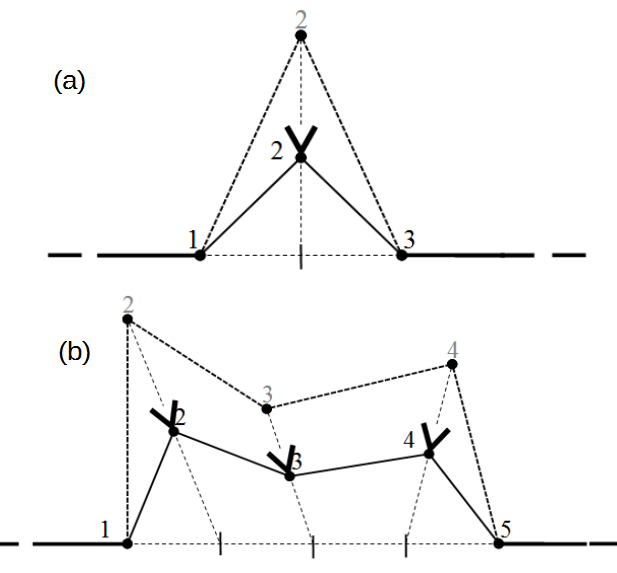
\includegraphics[height = 6cm]{images/manual_move_ctrl_pts.png}
    \caption[Method for moving manually the control points]{Method for moving manually the control points for a single manual move (a) and multiple moves (b)}
    \label{fig:manual_move_ctrl_pts}
\end{figure}

Then considering the $j^{th}$ line of the $A$ matrix which was too small, we now set the coefficients as follows:
$$ A[j][j] = 1,\ A_[j][\neq j] = 0,\ A_[\neq j][j] = 0 $$
$$ b[j] = 0 $$

\subsubsection{Stop conditions} \label{sec:stop_condition}

For each iteration (or loop) $l$ of the algorithm, an error term $\epsilon_l$ is computed as follows:

\begin{equation}
    \epsilon_l = \frac{1}{nb\_of\_points}\sum_k d_k^2
\end{equation}

Then, this squared average is compared to a threshold value and to the previous value of $\epsilon_l$ with $\epsilon_0 = +\infty$. If $\epsilon_l$ is lower than the threshold, the current B-spline is optimized and the algorithm stops. If $\epsilon_l > \epsilon_{l-1}$, the B-spline at the iteration $l-1$ is kept and the algorithm stops. Finally, if $l = l_{max}$, the algorithm stops and the last B-spline is saved.

\vsp

For a greater processing speed, the gradient of $\epsilon_l$ can be computed in order to stop the algorithm if the variation becomes too small.

\subsection{Point cloud generator}

In order to test the algorithm, a generator of point cloud has been implemented. It consists into drawing a circle with a few points, and randomizing their position around a perfect circle. Then points are generated all around the curve following a normal law.

\vsp

The figure \ref{fig:shape_gen_examples} shows different shapes generated for testing purpose. Various parameters like the standard deviation errors of the data points and shape points and the number of edges are tested in those examples. 

\begin{figure}[H]
    \centering
    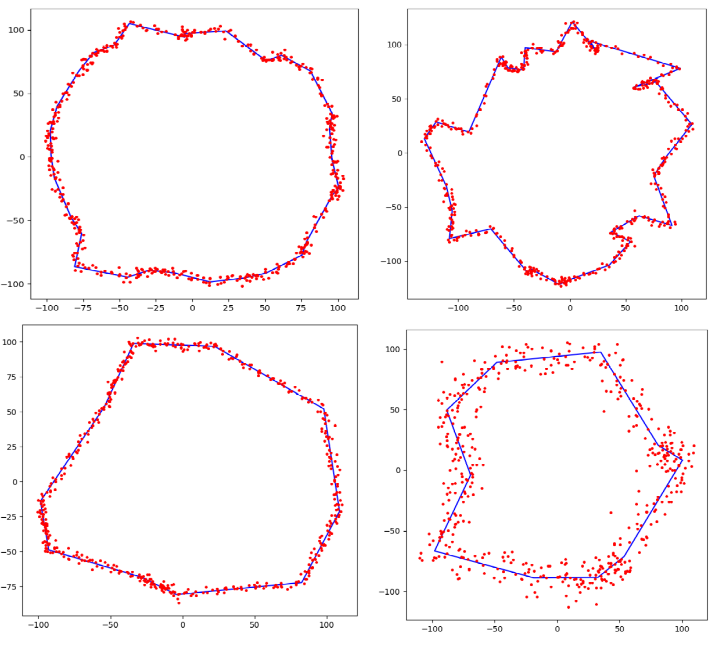
\includegraphics[width=7cm]{images/shape_gen_examples.png}
    \caption[Examples of generated testing shapes]{Examples of generated testing shapes with the raw shape in \textcolor{blue}{blue} and the data points in \textcolor{red}{red}}
    \label{fig:shape_gen_examples}
\end{figure}


\subsection{Results}

This section will describe the results of this method and some improvements that can be done.

\subsubsection{Testing}

All along this section, we will try to fit a point cloud and varying:

\begin{itemize}
    \item The ration $\frac{n}{p}$ with $n$ the number of control points and $p$ the number of point in the cloud
    \item The pondering factor $\lambda$ of the regularization term
    \item The sharpness of the point cloud
\end{itemize}

First the figure \ref{fig:bsp_res_general} shows what the result looks like. It has reached its minimum error in 1 iteration. 

\begin{figure}[H]
    \centering
    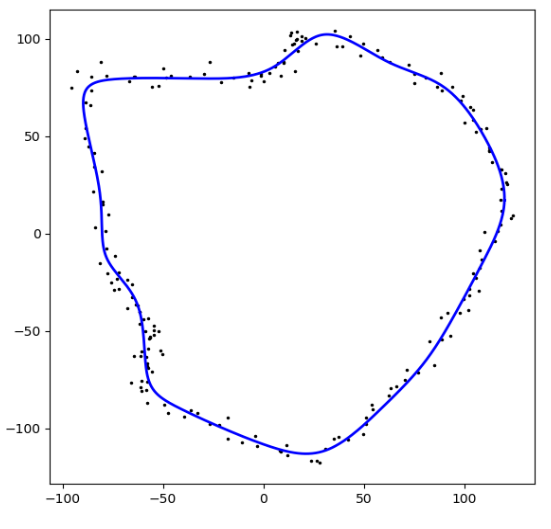
\includegraphics[width=5cm]{images/bsp_res_general.png}
    \caption[B-spline fitting in a basic point cloud]{B-spline fitting in a basic point cloud (n=20, p=200, $\lambda$=0.1)}
    \label{fig:bsp_res_general}
\end{figure}

\subsubsection{Influence of the number of control points} \label{sec:influence_n}

The figure \ref{fig:bsp_res_ctrl_pts} displays several curve reconstruction processes for various number of control points.

\begin{figure}[H]
    \centering
    \subfloat[5 control points] {
        \label{fig:bsp_res_ctrl_pts_5}
        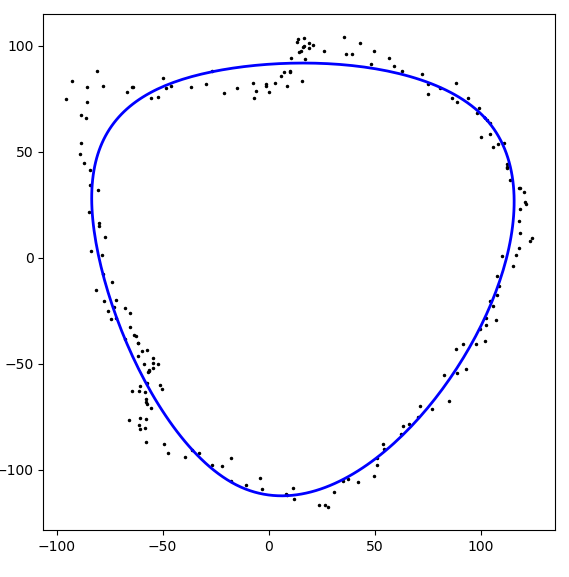
\includegraphics[width=5cm]{images/bsp_res/ctrl_pts/5.png}
        }
    \subfloat[10 control points] {
        \label{fig:bsp_res_ctrl_pts_10}
        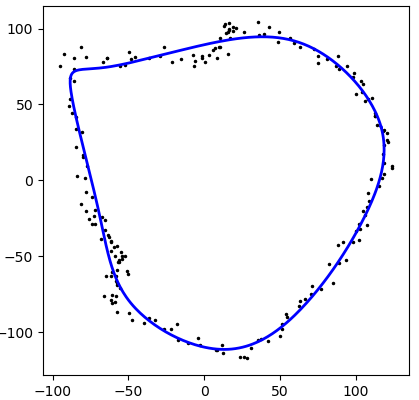
\includegraphics[width=5cm]{images/bsp_res/ctrl_pts/10.png}
        }
    \subfloat[20 control points] {
        \label{fig:bsp_res_ctrl_pts_20}
        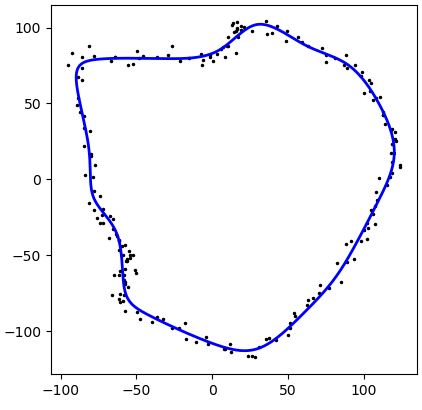
\includegraphics[width=5cm]{images/bsp_res/ctrl_pts/20.png}
        } \\
    \subfloat[40 control points] {
        \label{fig:bsp_res_ctrl_pts_40}
        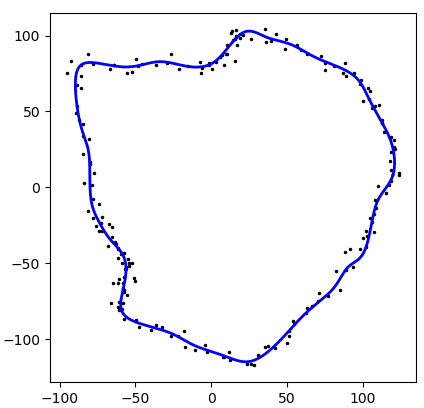
\includegraphics[width=5cm]{images/bsp_res/ctrl_pts/40.png}
        }
    \subfloat[80 control points] {
        \label{fig:bsp_res_ctrl_pts_80}
        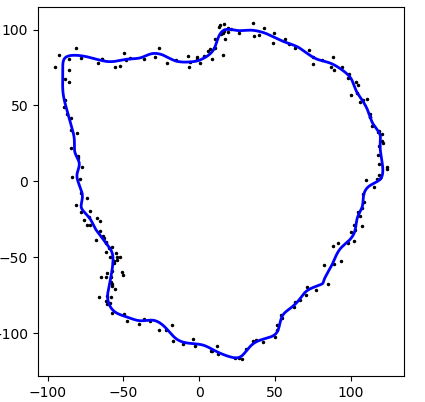
\includegraphics[width=5cm]{images/bsp_res/ctrl_pts/80.png}
        }
    \caption[Influence of the number of control points on the curve]{Influence of the number of control points on the curve (p=200, $\lambda$=0.1)}
    \label{fig:bsp_res_ctrl_pts}
\end{figure}

The number of control points describes the roughness of the shape. In our case, we want a high degree of precision on the body but if the data points become too few or too noisy, we will face an over-fitting problem as on the curve \ref{fig:bsp_res_ctrl_pts_80}. However, choosing too few control points won't be enough to fit the contour of the human waist, as on the curve \ref{fig:bsp_res_ctrl_pts_5} that is barely a round shape. 15 control points seem to be great for our purpose. 

\subsubsection{Influence of the regularization coefficient's value} \label{sec:influence_lambda}

Tests with several regularization coefficient's value are shown in figure \ref{fig:bsp_res_lambda}.

\begin{figure}[H]
    \centering
    \subfloat[$\lambda$=0.01] {
        \label{fig:bsp_res_lambda_0-01}
        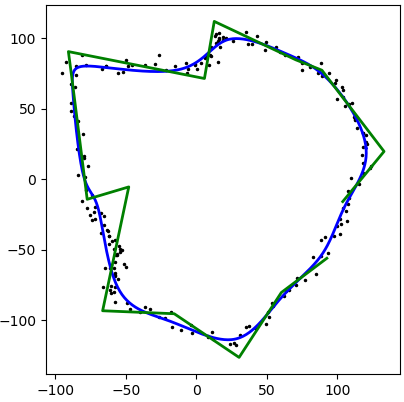
\includegraphics[width=5cm]{images/bsp_res/lambda/0-01.png}
        }
    \subfloat[$\lambda$=0.1] {
        \label{fig:bsp_res_lambda_0-1}
        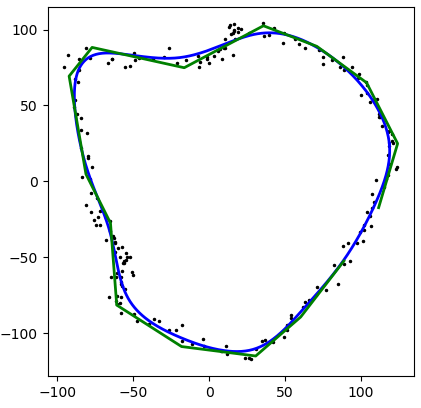
\includegraphics[width=5cm]{images/bsp_res/lambda/0-1.png}
        } 
    \subfloat[$\lambda$=10] {
        \label{fig:bsp_res_lambda_10}
        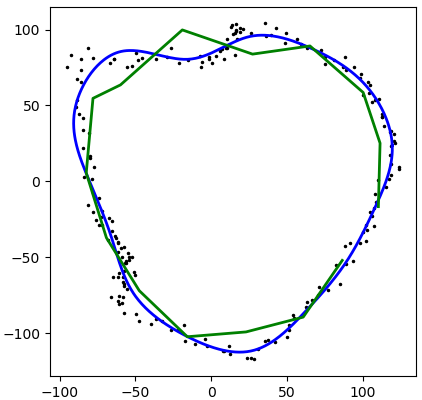
\includegraphics[width=5cm]{images/bsp_res/lambda/10.png}
        } 
    \caption[Influence of regularization coefficient's value on the curve]{Influence of regularization coefficient's value on the curve (n=15, p=200). The control points are shown in \textcolor{green}{green} while the curve is in \textcolor{blue}{blue}}
    \label{fig:bsp_res_lambda}
\end{figure}

As we expected, the higher the $\lambda$'s value, the more the curve will tend to minimize its circumference, i.e. becoming a circle. 

\subsubsection{Influence of the sharpness of the point cloud}

The figure \ref{fig:bsp_res_sharpness} shows the curve fitting for low, high and both point density:

\begin{figure}[H]
    \centering
    \subfloat[Low and high density point cloud] {
        \label{fig:bsp_res_sharpness_1}
        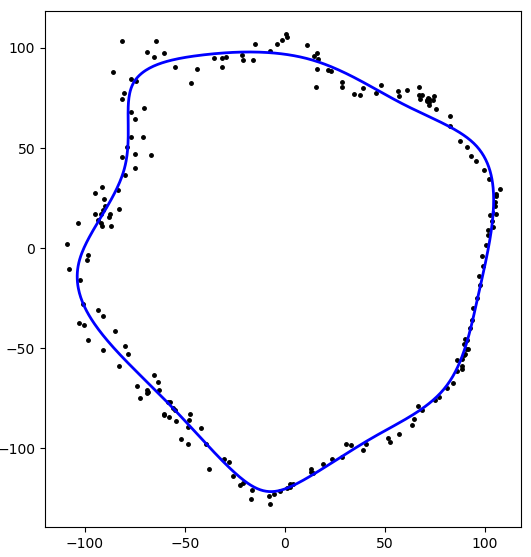
\includegraphics[width=5cm]{images/bsp_res/sharpness/test1.png}
        }
    \subfloat[Low density point cloud] {
        \label{fig:bsp_res_sharpness_2}
        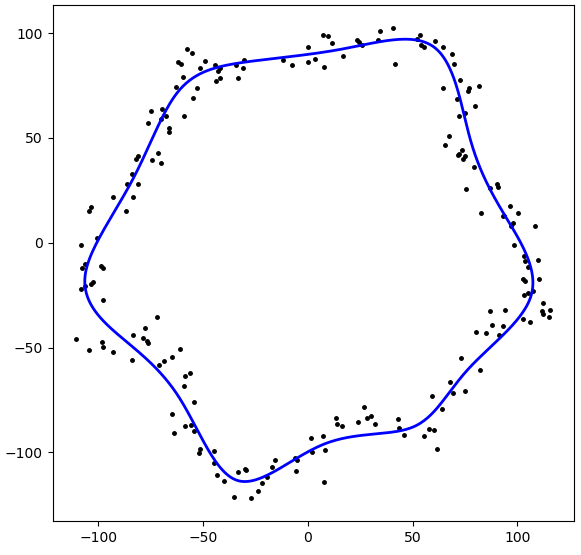
\includegraphics[width=5cm]{images/bsp_res/sharpness/test2.png}
        } 
    \subfloat[High density point cloud] {
        \label{fig:bsp_res_sharpness_3}
        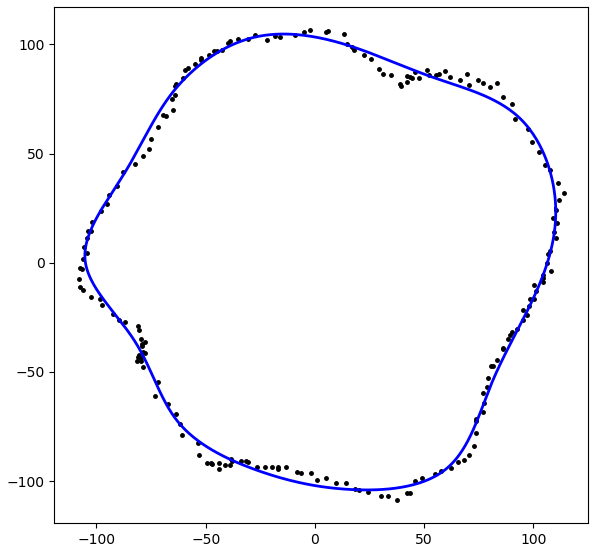
\includegraphics[width=5cm]{images/bsp_res/sharpness/test3.png}
        } 
    \caption[Influence of point cloud's sharpness on the curve]{Influence of point cloud's sharpness on the curve (n=15, p=200, $\lambda$=0.1)}
    \label{fig:bsp_res_sharpness}
\end{figure}

The results are quite satisfying as the curve always fit with the data. When the density is quite low as on the figure \ref{fig:bsp_res_sharpness_2}, a few number of control points is required, contrary to the figure \ref{fig:bsp_res_sharpness_3} where we notice that the curve is lacking of control nodes to fit perfectly with the data.

\subsubsection{Outliers detection} \label{sec:outlier_res}

The figure \ref{fig:bsp_res_outlier} shows clearly that the outliers detection works great when they are few enough. However, it won't work if the initial B-spline is fitted close to them.

\begin{figure}[H]
    \centering
    \subfloat[Without outliers detection] {
        \label{fig:bsp_res_outlier_without_detection}
        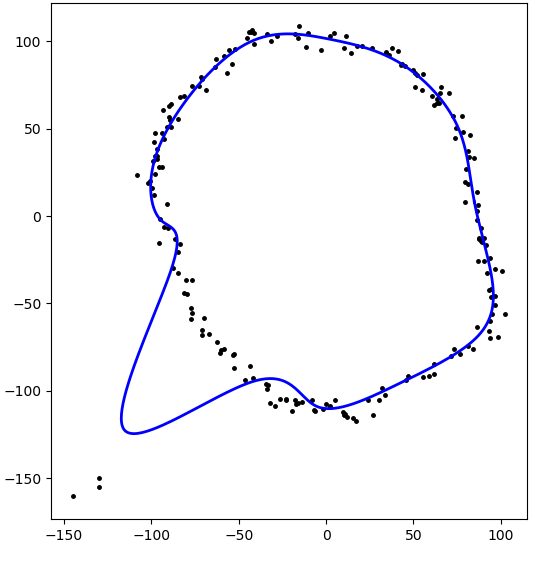
\includegraphics[width=5cm]{images/bsp_res/outlier/without.png}
        }
    \subfloat[With outliers detection] {
        \label{fig:bsp_res_outlier_with_detection}
        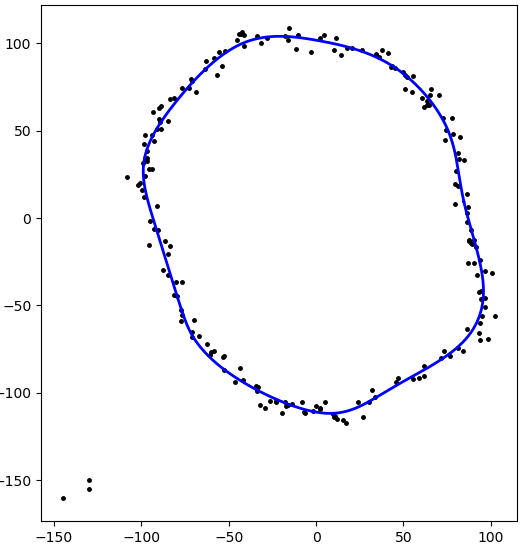
\includegraphics[width=5cm]{images/bsp_res/outlier/with.png}
        } 
    \caption[Test of the outlier detection]{Test of the outliers detection (n=15, p=200, $\lambda$=0.1)}
    \label{fig:bsp_res_outlier}
\end{figure}

\subsubsection{Possible improvements}

Several issues occurred while testing this solution. 

\vsp

First, if the set of data is becoming large or if the desired number of control points is too high, the algorithm can take a lot of time to run. A solution could be to run the program on a faster microprocessor or too run the algorithm with multiple threads. 

\vsp

It appears also that sometime, the number of control points is not well adapted to the shape (as seen in the section \ref{sec:influence_n}). A paper from Yang et al \cite{adjustement_ctrl_points} presents a method to increase or decrease the number of control points at each iteration until the desired error becomes lower than the objective.

\vsp

Moreover, it could be a great idea to implement an improved outliers detection as the currently implemented one is not robust to an high outlying points.

\vsp

Finally, a better regularization function should be integrated, bringing probably better results. Indeed, the current one only take in account the control points' position instead of the B-spline curve. 


\section{Running the program from a computer}

It is possible to run the whole program without accessing to the Raspi GUI's remotely.

\subsection{User's manual}

A serial bus is connected to the Raspi, and a USB-TTL converter allows the user to plug it to a computer. The program is run automatically at the Raspi's start-up and any terminal can be used to interact with it. Notice that the baudrate should be configured to 19200 and a constant should be set to \textit{True} to tell the Raspi to print and read on the serial. Finally, an other constant must be set to \textit{False} to avoid the Raspi showing the plot when using the serial.  

\subsection{Implementation}

The printing and reading functions have been overrode in order to choose where to read or print (serial or console). 

\vsp

Moreover, as the RX/TX ports are already taken by the servomotors serial, simple GPIO's are used and the serial is emulated in the software by a bitbang library. Thus, the baudrate cannot be set higher as the speed is limited by the CPU's speed.  

% List of figures & tables, biblio
\newpage
\listoffigures
\listoftables


\newpage
\bibliography{./references}
\bibliographystyle{ieeetr}

\end{document}